\chapter{Expectation-maximization algorithm}

The generic framework for expectation-maximization (EM) algorithms introduced
by \cite{bucstuvog15} applies to both language models and translation models.
This chapter will introduce terminology and notation from \cite{bucstuvog15} as
far as is necessary to apply this framework to the Hidden Markov Model in the
subsequent chapters.

\section{Preliminaries}

The set $\brc{0,1,2,\ldots}$ of non-negative integers and the set of
non-negative reals shall be denoted by $\zn$ and $\zr_{\geq0}$, respectively.
We assume that
\begin{align*}
 0^0 &:= 1, &
 \log 0 &:= -\infty, &
 0 (-\infty) &= \log 0^0 = 1.
\end{align*}

\begin{definition}
 Given a countable set $X$, a mapping $c: X \to \zr_{\geq0}$ is called a \emph{$X$-corpus}.
\end{definition}

When used as input for a language model's training algorithm, $X$ is the set of
all sentences consisting of words from the language in question, and $c(x)$
describes how often a sentence $x\in X$ occurs in the corpus $c$. The
\emph{size} of the corpus is defined as
\begin{equation*}
 \abs c := \sum_{x\in X} c(x).
\end{equation*}

\begin{definition}
 A \emph{probability distribution of $X$} is an $X$-corpus of size 1.
\end{definition}

The set of all such probability distributions is denoted by $\um(X)$.
Probability distributions can be derived from corpora:

\begin{definition}
 Given a non-empty and finite $X$-corpus $c$, the \emph{empirical probability
 distribution} $\tilde c$ is defined as
 \[
  \tilde c(x) = \frac{c(x)}{\abs c}.
 \]
\end{definition}

This expression is not well-defined for $\abs c = 0$ or $\abs c = \infty$,
hence the requirement for $c$ to be non-empty and finite. If this cannot be
guaranteed, a fall-back function can be added.

\begin{definition}
 Given $p\in\um(X)$, a \emph{normalization mapping with fall-back $p$} is the mapping
 \[
  \overline p: \zr_{\geq0}^X \to \um(X),
  \quad
  c \mapsto \begin{cases}
   \tilde c & \text{if } 0 < \abs c < \infty, \\ p & \text{otherwise}.
  \end{cases}
 \]
\end{definition}

\begin{definition}
 Given an $X$-corpus $c$ and $p\in\um(X)$, the \emph{likelihood of $c$ under $p$} is
 \[
  p(c) := \prod_{x\in X} p(x)^{c(x)}.
 \]
\end{definition}

The likelihood describes the probability of observing the sentences from the
corpus $c$ when sentences occur with the probability distribution described by
$p$. A training algorithm will take $c$ as an input, and seek to find an
admissible $p$ such that $p(c)$ is maximized. If any $p$ is admissible, then
for non-empty and finite $c$, the optimal choice is $p = \tilde c$:

\begin{lemma}\label{lemma:empirical1}
 Let $c$ be a non-empty and finite $X$-corpus. Then $\tilde c(c) \geq p(c)$ for every $p\in\um(X)$.
\end{lemma}

\begin{proof}
 Since $\log$ is monotone, it suffices to show that $\log\tilde c(c) \geq \log p(c)$. Using Gibbs' inequality,
 \begin{align*}
  \log \tilde c(c)
  &= \sum_{x\in X} c(x) \cdot \log \tilde c(x)
  = \abs c \cdot \sum_{x\in X} \tilde c(x) \cdot \log \tilde c(x) \\
  &\geq \abs c \cdot \sum_{x\in X} \tilde c(x) \cdot \log p(x)
  = \sum_{x\in X} c(x) \cdot \log p(x)
  = p(c)
  \qedhere
 \end{align*}
\end{proof}

However, using $p = \tilde c$ directly is not useful because this probability
distribution is grossly overfitted: It will assign zero probability to any
sentence not in the original corpus. A useful language model thus limits the
set of admissible $p$ by describing the probability distribution in terms of
\emph{model parameters} $\omega\in\Omega$.

\begin{definition}
 Given a set $\Omega$, an \emph{$\Omega$-probability model for $X$} is a mapping $p:\Omega\to\um(X)$.
\end{definition}

Instead of $p(\omega)$, we write $p_\omega$. Training shall then find $\omega\in\Omega$ such that $p_\omega(c)$ is maximized.

\begin{definition}
 Given a set $\Omega$ and an $\Omega$-probability model $p$ for $X$, the
 \emph{maximum likelihood estimator} for $p$ is the mapping
 \[
  \mle_p: \zr_{\geq0}^X \to \up(\Omega),
  \quad
  c \mapsto \argmax_\omega p_\omega(c).
 \]
\end{definition}

$\mle_p(c)$ is the set of all $\omega$ with maximal likelihood, but training
only needs to find a single $\hat\omega \in \mle_p(c)$. Computing $\mle_p(c)$
by brute force is typically not tractible because the set $\Omega$ is infinite
(usually countably infinite). However, there is one easily solvable special
case.

\begin{lemma}\label{lemma:empirical2}
 Let $c$ be a finite $X$-corpus, and $p$ a $\Omega$-probability model for $X$.
 If there exists $\hat\omega\in\Omega$ such that $p_{\hat\omega} = \tilde c$,
 then $\hat\omega\in\mle_p(c)$.
\end{lemma}

\begin{proof}
 If $c$ is empty, then $p_\omega(c) = 1$ for every $\omega$, and thus $\mle_p(c) = \Omega \ni \hat\omega$. Otherwise, by Lemma~\ref{lemma:empirical1}, $p_{\hat\omega}(c) = \tilde c(c) \geq p_\omega(c)$ for every $\omega\in\Omega$, and thus $\hat\omega \in \mle_p(c)$.
\end{proof}

\section{Algorithmic skeleton}

\begin{algorithm}[t]
 \caption{Algorithmic skeleton for EM of language models according to \cite{bucstuvog15}}
 \label{alg:skeleton}
 \begin{algorithmic}[1]
  \algorithmheader[Input:] $X$-corpus $c$
  \algorithmheader         $\Omega$-probability model $p$ for $Y\times X$
  \algorithmheader         some initial parameter $\omega_0 \in \Omega_0$ where $\Omega_0 := \brc{\omega\in\Omega: p_\omega(c) \neq 0}$
  \algorithmheader[Implicit:] step mapping $\psi:\Omega_0\to\up(\Omega)$
  \algorithmheader            \hspace{1em} such that $\omega'\in\psi(\omega)$ implies $p_\omega(c) \leq p_{\omega'}(c)$
  \algorithmheader[Output:] sequence $\omega_1,\omega_2,\ldots\in\Omega_0$
  \algorithmheader            \hspace{1em} such that $p_{\omega_0}(c), p_{\omega_1}(c), p_{\omega_2}(c)$ nondecreasing

  \STATE $i\leftarrow 0$
  \WHILE{not converged}
   \STATE $\omega_{i+1} \leftarrow \text{select a member of $\psi(\omega_i)$}$
   \STATE output $\omega_{i+1}$
   \STATE $i\leftarrow i+1$
  \ENDWHILE
 \end{algorithmic}
\end{algorithm}

The major complication that occurs when trying to train a typical language
model is that not all required data is present in the corpus. For example, a
probabilistic context-free grammar is described by the probability distribution
of derivation rules. \cite{laryou90} When the training data consists of full
parse trees (\emph{supervized training}), the optimal probability distribution
can be found by simply counting how many times each rule is used across all
these parse trees, and then computing the empirical probability distribution
for this corpus. Most of the times, however, the training data will consist
only of sentences. The information about how to parse the sentences is hidden.

The same problem arises with the Hidden Markov Model: When training data is not
already annotated with state information, the information which states
correspond to which words from the training data remains hidden. Expectation
maximization algorithms can be used when parts of the training data are hidden
in such a way.

For the remainder, let
\begin{itemize}\setlength\itemsep{-0.3em}
 \item $X$ and $Y$ be countable sets,
 \item $\Omega$ be a set,
 \item $c$ be a finite $X$-corpus and
 \item $p$ be a $\Omega$-probability model for $Y\times X$.
\end{itemize}

$c$ represents the set of training data. Each $x\in\operatorname{supp}(c)$ is
an \emph{observation}. To judge its probability under a $p_\omega$, additional
\emph{hidden information} $y\in Y$ is required. For notational convenience, we define
\begin{align*}
 p_\omega(c) &:= \prod_{x\in X} p_\omega(x)^{c(x)}, &
 \text{where } p_\omega(x) &:= \sum_{y\in Y} p_\omega(x,y).
\end{align*}

That is, even though $p_\omega$ is a probability distribution over $Y\times X$,
we allow to take the likelihood of the $X$-corpus $c$ under $p$ by aggregating
the probabilities for all hidden information $y$ that lead to a certain
observation $x$.

The basic pattern for expectation maximization is outlined in
algorithm~\ref{alg:skeleton}. The algorithm starts with an initial $\omega_0$
such that $p_{\omega_0}(c) \neq 0$. It then iteratively employs a step mapping
to choose the next $\omega_i$ with a higher (or at least equal) likelihood than
the one that came before.

\begin{definition}
 A \emph{step mapping} is a mapping $\psi:\Omega_0\to\up(\Omega)$ which is nondecreasing in the following manner:
 \[
  \forall \omega\in\Omega_0: \forall \omega'\in\psi(\Omega): p_\omega(c) \leq p_{\omega'}(c)
 \]
\end{definition}

The step mappings that we will consider will typically consist of two steps:
\begin{enumerate}
 \item \emph{Expectation:} The training data $c$ is converted into a
  \emph{complete-data corpus}. Using the $\omega_i$ from the previous
  iteration, the complete-data corpus estimates how hidden information
  contributes to the observations in the original corpus.
 \item \emph{Maximization:} A suitable maximum-likelihood estimator is applied
  to the complete-data corpus to choose $\omega_{i+1}$.
\end{enumerate}

%TODO: this section may use some citations because it makes claims
This back and forth of using the current $\omega$ to enrich the training data
and using the enriched data to find a better $\omega$ will converge towards a
local maximum of likelihood. The iteration is therefore usually aborted after
the desired running time has been exceeded, or after the changes of
$p_{\omega_i}(c)$ per iteration have become smaller than some threshold.

\cite{bucstuvog15} identify three types of step mappings that build on each
other, each one more specific than the one before it. Since the training of
Hidden Markov Models will be identified as an instance of the most specific
step mapping, the remainder of this chapter will introduce all three in order.

\section{Corpus-based step mapping}

The most general type of complete-data corpus can be obtained by distributing
$c(x)$ among the hidden information $y$ according to the probability
distribution $p_\omega$:
\[
 c\!\dangle{\omega,p}(y,x) := \begin{cases}
  c(x) \cdot \frac{p_\omega(y,x)}{p_\omega(x)} & \text{if } p_\omega(x) \neq 0, \\
  0 & \text{if } p_\omega(x) = 0.
 \end{cases}
\]
Recall that $p_\omega(x) = \sum_y p_\omega(y,x)$. Therefore,
$\abs{c\!\dangle{\omega,p}} = \abs c$. This corpus now has the correct
structure for plugging it into $\mle_p$, yielding the \emph{corpus-based step
mapping}\footnote{The proof that this step mapping is nondecreasing can be
found in \cite[pp.~10]{bucstuvog15}.}
\[
 \stepmap p_\mathrm{cb}: \Omega_0\to\up(\Omega),
 \quad
 \omega \mapsto \mle_p\mbig\kla{c\!\dangle{\omega,p}} = \argmax_{\omega'} p_{\omega'}\mbig\kla{c\!\dangle{\omega,p}}.
\]

For very simple language models, the $\argmax$ can be solved at this point
already. To apply lemma~\ref{lemma:empirical2}, $\hat\omega$ needs to be found
such that $p_{\hat\omega} = \widetilde{c\!\dangle{\omega,p}}$. This operation
is typically hard, which is why a more specific step mapping is helpful.

\section{Simple counting step mapping}

The next such step mapping requires the language model to be described by a
\emph{counting information}. Before defining this term, some additional
notation needs to be introduced.

\begin{definition}
 Let $A$ and $B$ be sets. A mapping $p: B \to \um(A)$ is called
 \emph{conditional probability distributions of $A$ given $B$}. The set of all
 such mappings is denoted by $\um(A|B)$.
\end{definition}

To simply notation, we define $p(a|b) := p(b)(a)$.

\begin{definition}
 Let $C\subseteq A\times B$ be a set. Then
 \[
  \um_C(A|B) := \brc{p\in\um(A|B): \operatorname{supp}(p)\subseteq C}
 \]
 is the set of all conditional probability distributions of $A$ given $B$
 constrained to $C$.
\end{definition}

\begin{definition}
 Given a set $\Omega$, a \emph{conditional $\Omega$-probability model for $A$
 and $B$ (constrained to $C$)} is a mapping $q:\Omega\to\um(A|B)$ (or
 $q:\Omega\to\um_C(A|B)$).
\end{definition}

When talking about counting informations (and inside-outside informations in
the next section), we assume the previously established requirements for $X$,
$Y$, $\Omega$, $c$ and $p$. Furthermore, we require that $X$ and $Y$ both
contain a special symbol $\bot$ such that $c(\bot) = 0$. $\bot$ can easily be
added to any previously defined $X$ and $Y$ without affecting the requirement
for countability. The notation $U_{\not\bot} := U\setminus\brc\bot$ shall be
defined for any set $U$.

\begin{definition}
 Let $A$, $B$ and $C$ be sets such that $C\subseteq A\times B$. A
 \emph{counting information} is a triple $\varkappa = (q,\lambda,\pi)$ such
 that
 \begin{align*}
  q &: \Omega\to\um_C(A|B), &
  \lambda &: X_{\not\bot} \times Y_{\not\bot} \to [0,1], &
  \pi &: X_{\not\bot} \times Y_{\not\bot} \to \zr_{\geq0}^C.
 \end{align*}
\end{definition}

The motivation for this definition is to model hidden information $y$ as
consisting of countable events $c\in C$. $\lambda(x,y)$ describes whether (and,
possibly, with what probability) a certain $y$ can be the cause for a certain
observation $x$.\footnote{Most actual instances of $\lambda$ use only integer
images, i.~e.~$\lambda(X_{\not\bot}\times Y_{\not\bot}) = \brc{0,1}$, thus
following this intuitive notion. However, the possibility of using fractional
values for $\lambda(x,y)$ is occasionally useful, e.~g.~to define a counting
information for the IBM Model 1 in \cite[pp.~23]{bucstuvog15}.} For
$\lambda(x,y)>0$, $\pi(x,y)$ is a $C$-corpus that describes how often each
countable event occurs in this hidden information.

Following the assumption that the countable events $C$ fully encode the hidden
information $Y$, we can use these intuitive notions to describe the original
probability model $p$ in terms of the counting information.

\begin{definition}
 Given $\varkappa=(q,\lambda,\pi)$, the \emph{induced model} $\varkappa^\flat:\Omega\to\zr_{\geq0}^{Y\times X}$ is given by
 \[
  (\varkappa^\flat)_\omega(y,x) := \begin{cases}
   \lambda(x,y) \cdot q_\omega\mbig\kla{\pi(x,y)} & \text{if } x,y\neq\bot, \\
   1 - \sum_{x',y'\neq\bot} \lambda(x',y') \cdot q_\omega\mbig\kla{\pi(x',y')} & \text{if } x = y = \bot, \\
   0 & \text{otherwise}.
  \end{cases}
 \]
\end{definition}

This definition shows why the introduction of $\bot$ into $X$ and $Y$ was
useful. By defining $(\varkappa^\flat)_\omega(\bot,\bot)$ as above, we ensure
$\mnorm\abs{(\varkappa^\flat)_\omega} = 1$. Therefore, $\varkappa^\flat$ is an
$\Omega$-probability model for $Y\times X$ iff
$(\varkappa^\flat)_\omega(\bot,\bot) \geq 0$. We call $\varkappa$ \emph{proper}
in this case.

Since we now have a probability model $p = \varkappa^\flat$ as required by the
corpus-based step mapping, we can lift its complete-data corpus into the domain
of the counting information, obtaining a new complete-data corpus
\[
 c\!\dangle{\omega,\varkappa}: C \to \zr_{\geq0}, \quad
 (a,b) \mapsto \sum_{x,y} c\mnorm\dangle{\omega,\varkappa^\flat}(y,x) \cdot \pi(x,y)(a,b).
\]

We can now apply a maximum-likelihood estimator for $q$ to arrive at the step
mapping for this class of language models.

\begin{definition}
 Given a set $\Omega$ and a conditional $\Omega$-probability model $q$ for $A$
 and $B$, the \emph{conditional maximum likelihood estimator} for $q$ is the mapping
 \[
  \cmle_q: \zr_{\geq0}^{A\times B} \to \up(\Omega),
  \quad
  c \mapsto \argmax_\omega q_\omega(c).
 \]
\end{definition}

Using this definition, the \emph{simple counting step mapping}\footnote{The
proof that this step mapping is equivalent to
$\mnorm\stepmap{\varkappa^\flat}_\mathrm{cb}$, and thus also nondecreasing, can
be found in \cite[p.~13]{bucstuvog15}.} is
\[
 \stepmap\varkappa_\mathrm{sc}: \Omega_0 \to \up(\Omega), \quad
 \omega \to \cmle_q\mbig\kla{c\mnorm\dangle{\omega,\varkappa}} = \argmax_{\omega'} q_{\omega'}\mbig\kla{c\mnorm\dangle{\omega,\varkappa}}.
\]
The simple counting step mapping has two advantages over
$\stepmap\cdot_\mathrm{cb}$: First, many language models can be described in
terms of the countable events only, such that $\Omega = C$. In this case,
lemma~\ref{lemma:empirical2} can be used to solve the $\argmax$ by simply
computing the empirical probability distribution of
$c\!\dangle{\omega,\varkappa}$.

Second, even if this is not possible, the set of countable events $C$ is
usually much smaller than the set of all observations $X$ or hidden information
$Y$, making the evaluation of the $\argmax$ more tractable than for the
corpus-based step mapping. For example, when considering probabilistic
context-free grammars, $X$ (the set of all sentences) and $Y$ (the set of all
parse trees) are both countably infinite, but $C$ (the set of all derivation
rules) is finite.

\section{Regular tree grammars}

The third and most specific type of step mapping applies to language models
whose hidden information can be described as trees, such that the countable
events are labels in these trees' nodes. We therefore need to define a set of
terms regarding trees and tree grammars first.

\begin{definition}
 An \emph{alphabet} is a finite set.
\end{definition}

\begin{definition}
 Let $\Sigma$ be an alphabet and $V$ be a set. The \emph{set $U_\Sigma(V)$ of
 unranked trees over $\Sigma$ indexed by $V$} is the smallest set $T$ such that
 \[
  V \subseteq T \quad\wedge\quad \forall k\in\zn: \forall \sigma\in\Sigma, t_1,\ldots,t_k\in T: \sigma(t_1,\ldots,t_k)\in T.
 \]
\end{definition}

The notation $\sigma(t_1,\ldots,t_k)$ refers to the tree which has the label
$\sigma$ at its root and the subtrees $t_1,\ldots,t_k$ in that order. For
$k=0$, we shorten $\sigma() \equiv \sigma$. For $V=\emptyset$, we shorten
$U_\Sigma(\emptyset) \equiv U_\Sigma$. Trees from $U_\Sigma(V)$ have labels
from $\Sigma\cup V$ at each node, but labels from $V$ are only permitted at
leafs. For example, for $\Sigma = \brc{\sigma_1,\sigma_2}$ and
$V=\brc{v_1,v_2}$:

\[\begin{matrix}
 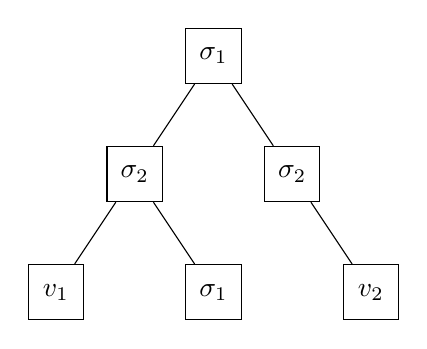
\begin{tikzpicture}[every node/.style={rectangle,draw,minimum size=2em},baseline=(current bounding box.center)]
  \node (n)   at (+0,+0.0) { $\sigma_1$ };
  \node (n1)  at (-1,-1.5) { $\sigma_2$ } edge (n);
  \node (n2)  at (+1,-1.5) { $\sigma_2$ } edge (n);
  \node (n11) at (-2,-3.0) { $v_1$ } edge (n1);
  \node (n12) at (+0,-3.0) { $\sigma_1$ } edge (n1);
  \node (n21) at (+2,-3.0) { $v_2$ } edge (n2);
 \end{tikzpicture}
 &\hspace*{4em}&
 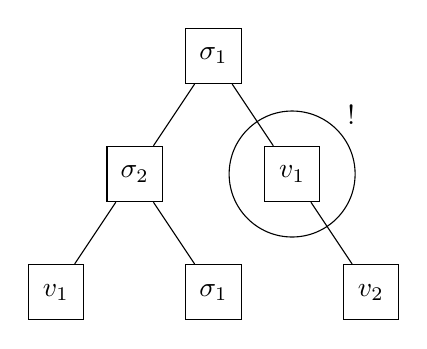
\begin{tikzpicture}[every node/.style={rectangle,draw,minimum size=2em},baseline=(current bounding box.center)]
  \node (n)   at (+0,+0.0) { $\sigma_1$ };
  \node (n1)  at (-1,-1.5) { $\sigma_2$ } edge (n);
  \node (n2)  at (+1,-1.5) { $v_1$ } edge (n);
  \node (n11) at (-2,-3.0) { $v_1$ } edge (n1);
  \node (n12) at (+0,-3.0) { $\sigma_1$ } edge (n1);
  \node (n21) at (+2,-3.0) { $v_2$ } edge (n2);
  \draw (n2) circle (0.8);
  \node[draw=none] at (+1.75,-0.75) {!};
 \end{tikzpicture}
 \\\\
 \sigma_1\mbig\kla{\sigma_2(v_1,\sigma_1), \sigma_2(v_2)} \in U_\Sigma(V) &&
 \sigma_1\mbig\kla{\sigma_2(v_1,\sigma_1), v_1(v_2)} \notin U_\Sigma(V)
\end{matrix}\]

We refer to positions in the tree using \emph{Gorn notation}. As a quick
illustration, in the figure below, each node of the left tree is labeled with
its position in the tree:

\vspace*{-1em}\[
 \hspace*{3em}
 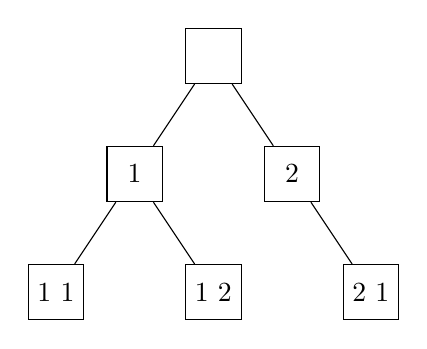
\begin{tikzpicture}[every node/.style={rectangle,draw,minimum size=2em},baseline=(current bounding box.center)]
  \node (n)   at (+0,+0.0) { $\eps$ };
  \node (n1)  at (-1,-1.5) { $1$ } edge (n);
  \node (n2)  at (+1,-1.5) { $2$ } edge (n);
  \node (n11) at (-2,-3.0) { $1\ 1$ } edge (n1);
  \node (n12) at (+0,-3.0) { $1\ 2$ } edge (n1);
  \node (n21) at (+2,-3.0) { $2\ 1$ } edge (n2);
 \end{tikzpicture}
 \hspace*{6em}
 \begin{tikzpicture}[baseline=(current bounding box.center)]
  \begin{scope}[every node/.style={rectangle,draw,fill=white,minimum size=2em}]
   \node (n)   at (+0,+0.0) { $\sigma_1$ };
   \node (n1)  at (-1,-1.5) { $\sigma_2$ } edge (n);
   \node (n2)  at (+1,-1.5) { $\sigma_2$ } edge (n);
   \node (n11) at (-2,-3.0) { $v_1$ } edge (n1);
   \node (n12) at (+0,-3.0) { $\sigma_1$ } edge (n1);
   \node (n21) at (+2,-3.0) {} edge (n2);
  \end{scope}
  \begin{scope}[every node/.style={inner sep=0},every pin/.style={inner sep=0},pin distance=1cm]
   \node[draw=none,pin=60:{$t(2\ 1)$}] at (n21.center) { $v_2$ };
  \end{scope}
  \begin{scope}[on background layer]
   \draw[line join=round,draw=black!10,fill=black!10,line width=1.5cm] (n1.center) -- (n11.center) -- (n12.center) -- cycle;
  \end{scope}
  \node at (-2.4,-1.7) { $t|_1$ };
 \end{tikzpicture}
\]

$\eps$ is the empty word. The set of all positions in a tree $t$ shall be
denoted by $\pos(t)$. The right tree illustrates some notation that we're going
to use for trees. For any trees $t,t'$ and position $w\in\pos(t)$,
\begin{itemize}\setlength\itemsep{-0.3em}
 \item $t(w)$ is the label at $w$,
 \item $t|_w$ is the subtree at $w$ (hence, especially, $t|_\eps = t$) and
 \item $t[t']_w$ is the tree that results from replacing $t|_w$ by $t'$.
\end{itemize}

\begin{definition}
 Let $\Sigma$ be an alphabet and $\square\notin\Sigma$. A \emph{1-context over
 $\Sigma$} is a tree $t\in U_\Sigma(\brc\square)$ such that $\square$ appears
 at exactly one position in $t$. The set of all such 1-contexts is denoted by
 $C_\Sigma$.
\end{definition}

1-contexts are used to describe trees that are not fully known yet: The
placeholder symbol $\sigma$ stands in for a missing subtree. Given a 1-context
$t\in C_\Sigma$ and a tree $t'\in U_\Sigma(V)$, we abbreviate $t[t'] :=
t[t']_w$ such that $t(w) = \square$. In other words, $t[t']$ is the tree that
results from $t$ when the $\square$ node is replaced by $t'$.

\begin{definition}
 A \emph{ranked alphabet} is a pair $(R,\rk)$ where $R$ is an alphabet and
 $\rk:R\to\zn$ is a mapping. $\rk$ is said to assign a \emph{rank} or
 \emph{arity} or each symbol in $R$.
\end{definition}

A ranked alphabet is usually denoted only by $R$. The existence of a suitable
$\rk$ is implied. A symbol $\rho\in R$ may be denoted as $\rho^{(k)}$ where
$\rk(\rho) = k$, to inform the reader of the symbol's rank.

\begin{definition}
 Let $R$ be a ranked alphabet and $V$ be a set. The \emph{set $T_R(V)$ of
 ranked trees over $R$ indexed by $V$} is defined by
 \[
  T_R(V) := \mbig\brc{t \in U_R(V) \dmiddle| \forall w\in\pos(t): \rk\mbig\kla{t(w)} = \text{number of children of $w$ in $t$}}.
 \]
\end{definition}

In other words, the number of children of each node in $t$ must be equal to the
rank of its label. For nodes labeled with symbols from $V$, a rank of 0 is
implied.

\begin{definition}
 Let $\Sigma$ be an alphabet. A \emph{regular tree grammar (RTG) over $\Sigma$} is a
 triple $\ug = (Q,q_0,R)$ where
 \begin{itemize}\setlength\itemsep{-0.3em}
  \item $Q$ is a nonempty alphabet (of states),
  \item $q_0\in Q$ is an initial state and
  \item $R\subset Q^*\times\Sigma\times Q$ is a finite ranked alphabet (of
   rules) such that every rule $\mbig\kla{(q_1,\ldots,q_k),\sigma,q}\in R$ has
   rank $k$.
 \end{itemize}
\end{definition}

We will write $\mbig\kla{(q_1,\ldots,q_k),\sigma,q}\in R$ as $q\to\sigma(q_1,\ldots,q_k)$ instead.

\begin{definition}
 Let $\ug=(Q,q_0,R)$ be an RTG over $\Sigma$. The \emph{family
 $\mbig\kla{D^q(\ug)\dmiddle|q\in Q}$ of partial abstract syntax trees oof
 $\ug$} is the smallest $Q$-indexed family $(D^q|q\in Q)$ such that, for all
 $q\in Q$,
 \[
  q \in D^q \quad\wedge\quad \forall \rho=\mbig\kla{q\to\sigma(q_1,\ldots,q_k)}\in R,d_i\in D^{q_i}: \rho(d_1,\ldots,d_k) \in D^q.
 \]
\end{definition}


An RTG describes a language (i.~e.~a countable set) of trees. Trees are derived
by starting with a tree containing only the a root node with the label $q_0$,
then successively replacing $Q$-labeled nodes according to the RTG's rule set
until no more $Q$-labeled nodes are left. The resulting tree is in $U_\Sigma$
and its syntax tree is in $T_R$. Partial syntax trees are in $T_R(Q)$.

For example, consider the RTG $\ug = \mbig\kla{\brc{q_0,q_1},q_0,R}$ where
$\Sigma=\brc{a,b,c}$ and
\[
 R = \brc{ q_0 \to a(q_0,q_1), \quad q_0 \to b, \quad q_1 \to c }.
\]
The tree $a(b,c)$ is derived like this: (Each row shows the partial tree $\in U_\Sigma(Q)$ on the left and the partial syntax tree $\in T_R(Q)$ on the right.)
\[\begin{matrix}
 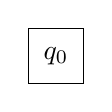
\begin{tikzpicture}[every node/.style={rectangle,draw,minimum size=2em},baseline=(current bounding box.center)]
  \node (n) at (0,0) { $q_0$ };
 \end{tikzpicture}
 &&
 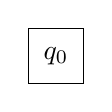
\begin{tikzpicture}[every node/.style={rectangle,draw,minimum size=2em},baseline=(current bounding box.center)]
  \node (n) at (0,0) { $q_0$ };
 \end{tikzpicture}
 \\\\[-1em]
 \downarrow & \text{apply } q_0\to a(q_0,q_1) & \downarrow \\[0.5em]
 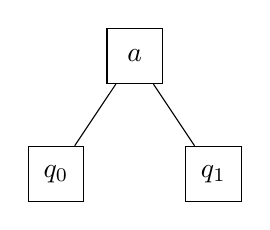
\begin{tikzpicture}[every node/.style={rectangle,draw,minimum size=2em},baseline=(current bounding box.center)]
  \node (n) at (0,0) { $a$ };
  \node (n1) at (-1,-1.5) { $q_0$ } edge (n);
  \node (n2) at (+1,-1.5) { $q_1$ } edge (n);
 \end{tikzpicture}
 &\hspace*{4em}&
 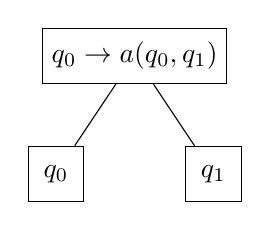
\begin{tikzpicture}[every node/.style={rectangle,draw,minimum size=2em},baseline=(current bounding box.center)]
  \node (n) at (0,0) { $q_0 \to a(q_0,q_1)$ };
  \node (n1) at (-1,-1.5) { $q_0$ } edge (n);
  \node (n2) at (+1,-1.5) { $q_1$ } edge (n);
 \end{tikzpicture}
 \\\\[-1em]
 \downarrow & \text{apply } q_0\to b & \downarrow \\[0.5em]
 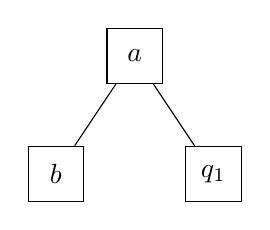
\begin{tikzpicture}[every node/.style={rectangle,draw,minimum size=2em},baseline=(current bounding box.center)]
  \node (n) at (0,0) { $a$ };
  \node (n1) at (-1,-1.5) { $b$ } edge (n);
  \node (n2) at (+1,-1.5) { $q_1$ } edge (n);
 \end{tikzpicture}
 &\hspace*{4em}&
 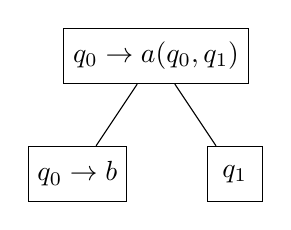
\begin{tikzpicture}[every node/.style={rectangle,draw,minimum size=2em},baseline=(current bounding box.center)]
  \node (n) at (0,0) { $q_0 \to a(q_0,q_1)$ };
  \node (n1) at (-1,-1.5) { $q_0\to b$ } edge (n);
  \node (n2) at (+1,-1.5) { $q_1$ } edge (n);
 \end{tikzpicture}
 \\\\[-1em]
 \downarrow & \text{apply } q_1\to c & \downarrow \\[0.5em]
 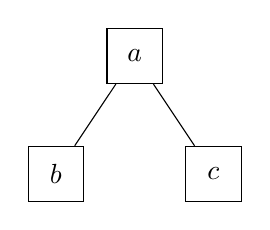
\begin{tikzpicture}[every node/.style={rectangle,draw,minimum size=2em},baseline=(current bounding box.center)]
  \node (n) at (0,0) { $a$ };
  \node (n1) at (-1,-1.5) { $b$ } edge (n);
  \node (n2) at (+1,-1.5) { $c$ } edge (n);
 \end{tikzpicture}
 &\hspace*{4em}&
 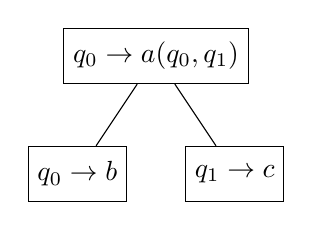
\begin{tikzpicture}[every node/.style={rectangle,draw,minimum size=2em},baseline=(current bounding box.center)]
  \node (n) at (0,0) { $q_0 \to a(q_0,q_1)$ };
  \node (n1) at (-1,-1.5) { $q_0\to b$ } edge (n);
  \node (n2) at (+1,-1.5) { $q_1\to c$ } edge (n);
 \end{tikzpicture}
\end{matrix}\]

From the syntax tree on the right, the tree on the left can be derived easily
by substituting the labels $q = \sigma(q_1,\ldots,q_k)\in R$ by the contained
symbols $\sigma\in\Sigma$. We shall call this projection $\pi_\Sigma: T_R(Q)\to U_\Sigma(Q)$.

\begin{definition}
 Let $\ug$ be an RTG over $\Sigma$. The \emph{language of $\ug$} is the set
 \[
  \lang\ug := \brc{t\in U_\Sigma | \exists d\in D^{q_0}(\ug): t=\pi_\Sigma(d)}.
 \]
 A language $L\subseteq U_\Sigma$ is \emph{recognizable} if there exists an RTG
 $\ug$ over $\Sigma$ such that $\lang\ug = L$.
\end{definition}

A useful property of RTGs is \emph{determinism}: An RTG $\ug$ over $\Sigma$ is
called \emph{deterministic} if, for any $(q_1,\ldots,q_k)\in Q^*$ and
$\sigma\in\Sigma$, there is at most one $q\in Q$ such that $\mbig\kla{q \to
\sigma(q_1,\ldots,q_k)} \in R$. A language is called deterministic if it is
described by a deterministic RTG.

From determinism results unambiguity: An RTG $\ug$ over $\Sigma$ is called
\emph{unambiguous} if, for every tree $t\in\lang\ug$, there exist exactly one
syntax tree $d\in D^{q_0}(\ug)$ such that $\pi_\Sigma(d) = t$. To see why, have
a look at the fully derived tree $t = a(b,c)$ above. Since $\ug$ in this
example is deterministic, the syntax tree can be recovered from $t$ by
traversing the nodes from the bottom up and assigning the rules that are used
at that position. At each position, we know the symbol $\sigma$ at this
position in the tree and the states $q_1,\ldots,q_k$ from the left sides of the
rules used for the child nodes. Therefore, the state $q$ (and therefore the
rule $\rho$) for this position can be chosen deterministically.

\begin{definition}
 A \emph{probabilistic regular tree grammar (PRTG) over $\Sigma$} is a pair
 $(\ug,p)$ of an RTG $\ug=(Q,q_0,R)$ over $\Sigma$ and a mapping $p:Q\to\zr_{\geq0}^{Q^*\times\Sigma}$ that is constrained to $R$ in the following way:
 \[
  \forall q\in Q, u\in Q^*\times\Sigma: p(q)(u) \neq 0 \Rightarrow (u,q) \in R.
 \]
 $(\ug,p)$ is called \emph{proper} if $p\in\um_R(Q^*\times\Sigma|Q)$. The
 \emph{meaning} of $(\ug,p)$ is the mapping
 \[
  \mbig\lang{(\ug,p)}: U_\Sigma \to \zr_0, \quad
  t \mapsto \sum_{d\in D^{q_0}(\ug): \pi_\Sigma(d)=t} p(d).
 \]
 Herein, $p(d) := p\mbig\kla{\pi(d)}$, where $\pi(d)$ is an $R$-corpus with
 \[
  \pi(d)(p) := \mbig\abs{\mbig\brc{w\in\pos(d): d(w)=p}}.
 \]
\end{definition}

We usually write a PRTG $(\ug,p)$ as just $\ug$ and imply the existence of $p$.
The meaning function assigns a probability to a tree from $\lang\ug$ by summing
the probability of all derivations resulting in that tree, where the
probability of a derivation is the product of the probability of each rule
occurring in it. This implies that each rule application is statistically
independent from each other.

{\color{red} TODO inside/outside weights, IO information, IO step mapping}
